\documentclass[conference]{IEEEtran}
\usepackage[T1]{fontenc}
\usepackage{cite}
\usepackage{amsmath,amssymb}
\usepackage{graphicx}
\usepackage{booktabs}
\usepackage{url}
\usepackage[hidelinks]{hyperref}
\usepackage{xcolor}
\usepackage{array,tabularx}
\usepackage{dblfloatfix}
\usepackage{balance}
\graphicspath{{figures/}}
\hypersetup{pdftitle={Reproduction and Extension of StockMixer for Stock Price Forecasting},pdfauthor={Kavin Karthik Yuvaraj},pdfsubject={Mini-Project Report}}
\newcommand{\HS}{HardSwish}
\newcommand{\sd}[2]{\ensuremath{#1\,\pm\,#2}}
\begin{document}
\title{Reproduction and Extension of StockMixer for Stock Price Forecasting}
\author{\IEEEauthorblockN{Kavin Karthik Yuvaraj}
\IEEEauthorblockA{Department of Computer Science and Engineering\\
Shiv Nadar University Chennai, India\\
Student ID: 24011101055\\
Email: \texttt{kavinkarthik24110077@snuchennai.edu.in}}}
\maketitle
\begin{abstract}
Stock-return forecasting combines temporal prediction with the ranking of stocks across a market. This project reproduces released StockMixer configurations and extends the training workflow with exact recording, recoverable checkpoints, execution optimizations, and stock-branch diagnostics. Experiments use supplied NASDAQ arrays containing 1,026 stocks and five features, with a 16-day lookback and one-day prediction horizon. The main comparison covers 21 completed runs and 2,100 training epochs, including three released-code activation arrangements and six modified configurations. The released GELU/GELU/HardSwish arrangement records mean daily Pearson correlation of 0.0408; the modified no-stock configuration reaches mean correlation 0.03517. Saved states allow numerical checks of mixed precision and checkpoint comparisons, while GPU preloading reduces repeated data transfers. A corrective investigation identifies sparse stock-branch activity associated with a large negative normalization-bias contribution. Freezing only this additive bias restores substantial activation coverage, but forecasting improvement varies across matched runs. The project provides recoverable training states and measurements linking execution choices, checkpoint selection, and stock-branch behavior. Project repository: \url{https://github.com/artemiskavin/Stock-Mixer}.
\end{abstract}
\begin{IEEEkeywords}
StockMixer, stock-return forecasting, reproducibility, mixed precision, normalization, model diagnostics
\end{IEEEkeywords}
\section{Introduction}
Next-day stock returns are noisy, nonstationary, and mutually dependent. Forecasting systems must capture temporal patterns and cross-stock relationships while supporting useful ranking decisions. Lower regression error need not improve selection of the highest-returning stocks, so evaluation requires both predictive and portfolio-oriented measures.

Fan and Shen's StockMixer combines indicator, temporal, and stock mixing through multilayer perceptrons and a market-width bottleneck~\cite{stockmixer}. Its compact architecture permits component comparisons and internal-state inspection on one graphics processor. The original paper provides the full derivation; this project concentrates on the executed implementation and completed experiments.

The released trainer prints rounded metrics but saves neither all-epoch weights nor resumable state. It also lacks stock-activation measurements. These omissions limit checkpoint and branch analysis. We retain the states and measurements needed to study the observed stock-mixing sparsity after training.

We compare released configurations with documented component removals and recurrent controls. A separate matched experiment examines how stock-axis normalization affects activation coverage and forecasting. GPU preloading and batched logging target transfer and synchronization costs while preserving the supplied data, author loss, and epoch budgets. Their runtime effects are measured separately from forecasting performance.

The contributions are:
\begin{itemize}
\item A completed NASDAQ comparison covering 21 main runs and 2,100 epochs, with consistent minimum-validation-loss reporting for saved checkpoints and recorded released-trainer results.
\item An instrumented workflow with exact epoch metrics, all-epoch weight retention, state-complete resumption, numerical compatibility gates, GPU preloading, and measured execution comparisons.
\item A stock-branch investigation that decomposes the effective normalization offset and tests a matched beta-zero intervention under corrected sampling and eager full precision.
\end{itemize}

\section{Related Works}
\subsection{Mixing Architectures}
MLP-Mixer alternates token- and channel-mixing perceptrons, enabling cross-location and cross-feature communication without attention or convolution in its vision setting~\cite{mlpmixer}. Its image-token construction motivates matrix-based mixing but does not encode financial temporal order or market structure.

StockMixer adapts mixing to indicators, multi-scale temporal representations, and stock-to-market-to-stock exchange~\cite{stockmixer}. The paper evaluates NASDAQ, NYSE, and S\&P500 with ablations and sensitivity studies. We reproduce the NASDAQ implementation and extend observable training behavior within a smaller computational scope.

\subsection{Temporal and Relational Baselines}
Long short-term memory networks propagate information through gated recurrent state~\cite{lstm}; gated recurrent units provide a related state-update mechanism~\cite{gru}. They supply temporal controls here. Shared per-stock recurrent models do not explicitly exchange information across the universe, enabling comparison with architectures that add stock mixing.

Relational Stock Ranking combines ranking with temporal graph convolution over company relationships~\cite{rsr}. Its external relations and graph pipeline introduce requirements beyond a temporal encoder. Reconstructing the complete graph/hypergraph suite was outside our scope; LSTM, GRU, and LSTM plus stock mixing provide focused controls.

\subsection{Position of This Project}
We examine cross-stock activity using retained weights and matched normalization diagnostics. Numerical checks establish usable execution paths. The records support comparisons of activation coverage and forecasting performance at the selected states.

\section{Proposed Methodology}
\subsection{Problem Formulation and Dataset}
At position $t$, input $X_t\in\mathbb{R}^{N\times T\times F}$ contains $N=1026$ stocks, $T=16$ historical positions, and $F=5$ features. Predicted price $\hat p_i$ is converted to return using final base price $p_i^{\mathrm{base}}$:
\begin{equation}
\hat r_i=\frac{\hat p_i-p_i^{\mathrm{base}}}{p_i^{\mathrm{base}}}.
\label{eq:return}
\end{equation}
Supplied preprocessing, arrays, masks, and stock order are preserved. The 1,245 positions include validation targets 756--1007 and test targets 1008--1244 (237 days). The paper lists 273 test days; we use the dates in the released arrays.

Main reproduction experiments retain the released sampler: an offset array 0--755 is initialized once, shuffled in place each epoch, and its first 740 entries are used. Possible training targets are therefore 16--771, including 16 validation target positions. We retain this overlap for comparison with the released training procedure. Corrective diagnostics separately restrict offsets to 0--739 and targets to 16--755, excluding reused validation labels. Valid historical input context is retained across split boundaries. Data were not reprocessed to obtain improved scores.

\subsection{Architecture and Component Definitions}
Figure~\ref{fig:architecture} shows the executed full-model path from the released source~\cite{releasedcode}. A 16-step temporal/indicator path and a convolutionally downsampled 8-step path are combined with the raw temporal input. Their concatenation has 40 temporal positions. A shared feature projection produces $H\in\mathbb{R}^{1026\times40}$. One price head acts directly on $H$; another acts on its stock-mixed representation. Their price outputs are summed.

The stock mixer applies LayerNorm across the stock axis, projects 1,026 stock inputs to market width 20, applies an activation, and projects back to 1,026 outputs. Full StockMixer contains 45,077 parameters. The released arrangements use GELU in both indicator perceptrons and HardSwish, GELU, or Sigmoid in the stock perceptron. In the modified matrix, surviving mixing perceptrons use HardSwish and recurrent gates remain native.

The no-indicator variant bypasses both indicator-perceptron residual terms. The no-TriU variant removes triangular temporal mixing. The convolution and remaining temporal paths are retained. The no-stock variant removes both the stock branch and its price head. LSTM and GRU have one shared recurrent layer with hidden size 32; the LSTM-plus-stock model adds the documented stock mixer and associated head. These definitions are fixed across repetitions. Full construction precedes parameter-free pruning where applicable, preserving common initial parameter values and construction order.

\begin{figure*}[t]
\centering
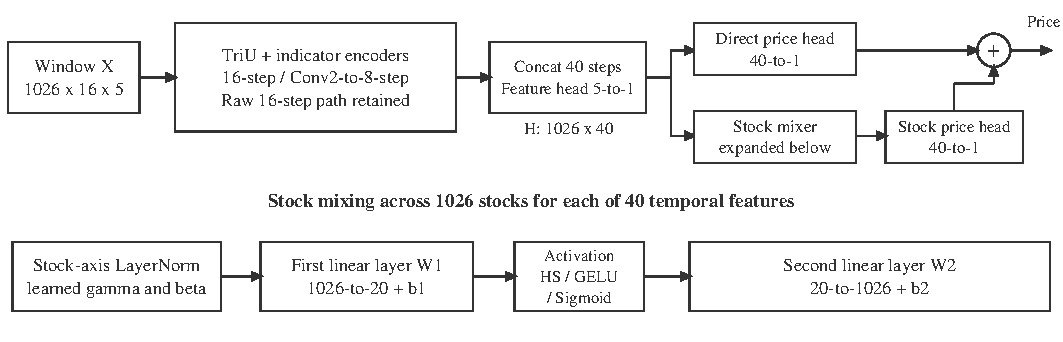
\includegraphics[width=\textwidth]{architecture.pdf}
\caption{Executed full StockMixer forward path and expanded stock mixer. The direct and stock price heads are added at the output. HS denotes HardSwish. The raw temporal branch and stock-axis dimensions follow the released source.}
\label{fig:architecture}
\end{figure*}

\subsection{Author Loss and Frozen Checkpoint Rules}
For validity mask $m_i$ and realized return $r_i$, the retained objective is
\begin{align}
\mathcal L_{\mathrm{MSE}}&=\frac{1}{N}\sum_i[m_i(\hat r_i-r_i)]^2,\\
\mathcal L_{\mathrm{rank}}&=\frac{1}{N^2}\sum_{i,j}
\left[-(\hat r_i-\hat r_j)(r_i-r_j)m_i m_j\right]_+,\\
\mathcal L&=\mathcal L_{\mathrm{MSE}}+0.1\mathcal L_{\mathrm{rank}},
\label{eq:loss}
\end{align}
where $[a]_+=\max(0,a)$. The full-$N$ and full-$N^2$ denominators are preserved. They differ from the evaluator's valid-observation MSE denominator. Each full-market update forms a $1026\times1026$ ranking matrix, explaining appreciable computation despite the compact parameter count.

Every main run completes 100 epochs without early stopping. Adam uses learning rate 0.001, betas $(0.9,0.999)$, epsilon $10^{-8}$, zero weight decay, and no AMSGrad. Saved checkpoints are reported using minimum validation combined loss. Released-trainer rows retain previously recorded rounded-console metrics; console precision does not establish an exact recoverable checkpoint. Modified rows report arithmetic means and sample standard deviations across completed repetitions. Initialization uses the predefined NumPy/PyTorch seed pairs 123456789/12345678, 234567890/23456789, and 345678901/34567890 as applicable to the executed configuration.

The alternative frozen selection uses
\begin{align}
\mathcal E&=\{e:\mathcal L_{\mathrm{val}}(e)\leq1.10\mathcal L_{\min}\},\\
e_{\mathrm{IC}}&=\underset{e\in\mathcal E}{\arg\max}\;\mathrm{IC}_{\mathrm{val}}(e),
\label{eq:selection}
\end{align}
with exact ties broken by lower validation loss, then earlier epoch. The comparison tables consistently use lowest-loss results. Test metrics do not choose checkpoints, execution settings, or continuation.

\subsection{Reproducible Recording and Efficient Execution}
The workflow saves exact epoch metrics, all 100 weight states, and selection metadata. Resumable LAST state retains model, optimizer, RNG, offset permutation, modes, existing gradients, and AMP scaler where applicable. Source/data hashes identify configurations; preservation checks guard scientific state during recording and diagnostics. These recording, execution, and diagnostic extensions are retained in the project archive~\cite{project}.

Figure~\ref{fig:workflow} outlines the execution pipeline. Features, masks, base prices, and targets are transferred to the GPU once. Windows are sliced there using the unchanged shuffled order, avoiding repeated construction and transfer of four CPU tensors per update. Detached losses and predictions are buffered on device and transferred in batches, reducing synchronization while preserving aggregation order.

Automatic mixed precision (AMP) uses FP16 for eligible model operations. Model parameters, price heads, return conversion, and loss remain FP32; GradScaler supports the backward computation. Fifteen retained modified runs use AMP. GRU uses FP32 because its fixed-state FP16 gradient comparison gave relative $L_2$ error 0.592 and cosine 0.811, failing the fixed 0.05/0.99 gates. Compilation is applied only where numerical checks pass. No-indicator and no-TriU use eager seed-0 execution and compilation later; no-stock and LSTM-plus-stock use compilation. LSTM/GRU compile supported heads while retaining native recurrent cells. The modified pipeline disables TF32; released-code runs inherit installed defaults.

\begin{figure*}[t]
\centering
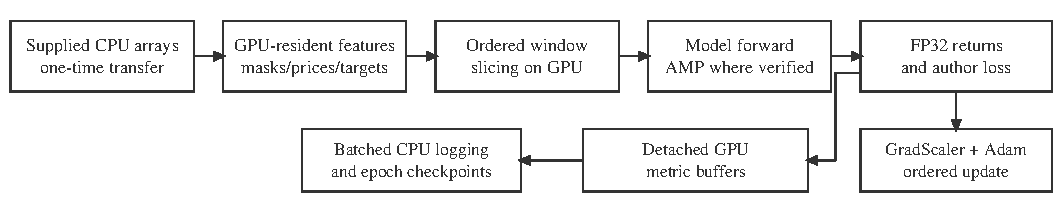
\includegraphics[width=\textwidth]{gpu_workflow.pdf}
\caption{GPU-resident execution, ordered window updates, and batched recording. AMP/GradScaler are bypassed for FP32 conditions. The optimizations target transfer, synchronization, and execution overhead; measured timing is reported separately.}
\label{fig:workflow}
\end{figure*}

\subsection{Stock-Branch Diagnostic and Matched Intervention}
For stock-axis normalization, the first hidden preactivation can be decomposed as
\begin{align}
\operatorname{LN}(x)&=\gamma\odot\bar x+\beta,\\
z&=W_1(\gamma\odot\bar x)+(W_1\beta+b_1),
\label{eq:offset}
\end{align}
where $\bar x$ is the standardized stock-axis input. The constant term $W_1\beta+b_1$ is distinct from total preactivation. Each hidden unit sums 1,026 weighted beta contributions; aligned signs can create a large shift even if individual terms are small. HardSwish has zero output for preactivation at or below $-3$, so the fraction below that boundary measures an inactive portion of the gate.

Corrected-sampler diagnostics train fresh all-HardSwish full models in eager FP32 for 100 epochs. The matched intervention freezes only the existing stock-axis LayerNorm bias beta at its initial zero value. Gamma and every other parameter remain trainable. Common initial tensors and per-epoch shuffle hashes are checked. Fixed probes, preactivation distributions, effective offsets, active-unit/window coverage, and branch-gradient norms are retained without changing training state. Selected states receive full training/validation activation censuses. We then compare their forecasting results to determine whether restored activity accompanies a predictive gain.

\subsection{Implementation Details and Project Scope}
Experiments run on a Lenovo laptop with Intel Core i5-12450H (8 cores/12 threads), 16 GB RAM, and an NVIDIA RTX 4060 Laptop GPU with 8 GB VRAM. The environment is Windows 11, Python 3.10.21, PyTorch 2.9.1+cu128, CUDA runtime 12.8, cuDNN 9.10.2, NumPy 1.22.1, and NVIDIA driver 617.42. These settings describe our installed environment. The paper used a different historical software stack.

NASDAQ-only evaluation keeps the repeated matrix and diagnostics manageable on one GPU. NYSE/S\&P500 expansion, the complete graph/hypergraph baseline suite, broad lookback/market-width/scale searches, and ReLU/tanh sweeps are outside the completed scope. External relation preprocessing and exact paper ablation sources were not supplied with the preserved release. Effort was allocated to repeated modified configurations, retained artifacts, execution checks, and matched mechanism tests. The linked repository contains the selected implementations and reproduction instructions.

\section{Results and Discussion}
\subsection{Experimental Setup and Evaluation}
The main comparison covers 21 completed 100-epoch runs: three released-code activation configurations and six repeated modified configurations. Table~\ref{tab:mainresults} identifies recorded console values and saved selections. All comparisons use the same released-array test positions; follow-up evidence is not a newly reserved evaluation period.

Information coefficient (IC) is the official evaluator's mean daily Pearson correlation across stocks. Official-code RIC is the daily Pearson IC information ratio (mean divided by population standard deviation), not Spearman correlation. Precision@10 is the fraction of nonnegative realized returns among the selected top ten valid stocks. Gross Sharpe@5 uses equal-weight top-five returns, mean/population standard deviation times 15.87, without transaction costs. Evaluator MSE is a valid-mask average of squared return-prediction error. It is separate from both the training MSE component and combined author loss.

\begin{table*}[t]
\centering
\caption{Forecasting results. Released-trainer rows retain rounded recorded metrics; modified rows are arithmetic means $\pm$ sample SD from lowest-validation-loss saved states. Evaluator MSE is multiplied by $10^4$ and P@10 is a percentage.}
\label{tab:mainresults}
\small
\setlength{\tabcolsep}{4pt}
\begin{tabular}{@{}lrrrrrr@{}}
\toprule
Configuration & Params & IC & Official RIC & MSE $\times10^4$ & P@10 (\%) & Gross SR@5\\
\midrule
\multicolumn{7}{l}{\textit{Recorded released-trainer results}}\\
GELU / GELU / HardSwish & 45,077 & 0.0408 & 0.482 & 3.94 & 54.8 & 1.62\\
GELU / GELU / GELU & 45,077 & 0.0368 & 0.414 & 3.94 & 53.5 & 1.72\\
GELU / GELU / Sigmoid & 45,077 & 0.0225 & 0.242 & 4.61 & 53.0 & 0.356\\
\midrule
\multicolumn{7}{l}{\textit{Modified configurations: mean $\pm$ sample SD}}\\
Without indicator mixing & 44,957 & \sd{0.02764}{0.00510} & \sd{0.328}{0.042} & \sd{4.115}{0.394} & \sd{51.69}{0.89} & \sd{0.812}{0.981}\\
Without TriU mixing & 44,881 & \sd{0.01987}{0.01569} & \sd{0.263}{0.188} & \sd{3.915}{0.110} & \sd{51.32}{0.52} & \sd{0.896}{1.075}\\
Without stock mixing & 898 & \sd{0.03517}{0.00591} & \sd{0.459}{0.099} & \sd{3.867}{0.044} & \sd{52.38}{0.79} & \sd{1.128}{0.510}\\
LSTM & 5,025 & \sd{0.02751}{0.00531} & \sd{0.300}{0.055} & \sd{3.792}{0.007} & \sd{51.69}{0.58} & \sd{0.395}{0.544}\\
GRU & 3,777 & \sd{0.02875}{0.01140} & \sd{0.300}{0.117} & \sd{3.787}{0.004} & \sd{52.15}{0.81} & \sd{-0.372}{0.440}\\
LSTM plus stock mixing & 49,196 & \sd{0.02365}{0.00801} & \sd{0.284}{0.089} & \sd{3.824}{0.069} & \sd{51.32}{1.13} & \sd{-0.054}{1.285}\\
\bottomrule
\end{tabular}
\end{table*}





\subsection{Quantitative Forecasting Results}
The released GELU/GELU/HardSwish arrangement records the strongest displayed IC (0.0408), official RIC (0.482), and Precision@10 (54.8\%) among its three arrangements. All-GELU records the highest gross Sharpe (1.72). The Sigmoid arrangement records IC 0.0225 and gross Sharpe 0.356. The strongest full-market correlation and highest top-five Sharpe occur in different arrangements. Test performance was not used to select an activation.

Figure~\ref{fig:ic_overview} summarizes the IC comparison. Within the modified group, the 898-parameter no-stock model achieves the largest mean IC (0.03517), official RIC (0.459), and gross Sharpe (1.128). Variation across repetitions is greatest for no-TriU, whose IC sample SD reaches 0.01569. GRU gives the lowest evaluator MSE. Its negative mean gross Sharpe shows weak top-five portfolio performance despite low average return-prediction error. These experiments used different implementation settings. Results are exploratory, and differences across groups cannot be attributed solely to removing model components.

IC measures daily cross-sectional association and is unchanged by positive rescaling within a day. MSE additionally penalizes calibration and prediction magnitude. Consequently, low return-prediction error need not imply a strong stock ranking. GRU has slightly higher mean IC than LSTM (0.02875 versus 0.02751), yet lower gross Sharpe ($-0.372$ versus 0.395). The latter depends on return magnitude and variability among only five selections. Precision@10 counts nonnegative outcomes without measuring their size. The metrics describe different aspects of the same predictions, so their rankings can differ.

For context, the paper reports NASDAQ StockMixer IC 0.043~\cite{stockmixer}, compared with 0.0408 in the released HardSwish run: a descriptive difference of 0.0022, or about 5.1\%. The paper describes RIC as Spearman correlation, whereas the released implementation uses the Pearson IC information ratio. This report follows the executed evaluator and does not treat the two RIC definitions as interchangeable.

\subsection{Execution and Checkpoint Findings}


Table~\ref{tab:timing} measures complete epochs, including work outside GPU kernels. Compiled warm medians fall by approximately 20\% for HardSwish and 38\% for Sigmoid. Startup makes the HardSwish compiled total longer overall. Different seeds and nonconcurrent runs prevent isolation of AMP, preloading, or compilation effects.

Preloading reduces repeated transfers, and batched recording reduces synchronization. AMP changes eligible arithmetic. Fixed numerical checks require FP32 for GRU. Table~\ref{tab:mainresults} reports forecasting performance separately.

A separate recording-only author-code comparison records test IC 0.02582928 against 0.04080 for the unchanged trainer, approximately 36.7\% lower. Source audit found recording/saving additions as the only source changes. This observation does not establish that recording caused the difference: historical weights were unavailable and GPU determinism was not enforced.

The frozen 10\%-tolerance rule produces an even split against minimum-loss selection in the 18 retained modified runs: test IC improves in 9 and decreases in 9. These counts establish no overall benefit. The tolerance was unchanged; retained checkpoints permit analysis of the differences.

\begin{figure}[t]
\centering
\setlength{\unitlength}{0.01\columnwidth}
\begin{picture}(100,69)
\linethickness{0.25pt}
\put(43.000,14.000){{\color{black!15}\line(0,1){51}}}
\put(43.000,11.500){\makebox(0,0){\scriptsize 0.00}}
\put(53.800,14.000){{\color{black!15}\line(0,1){51}}}
\put(53.800,11.500){\makebox(0,0){\scriptsize 0.01}}
\put(64.600,14.000){{\color{black!15}\line(0,1){51}}}
\put(64.600,11.500){\makebox(0,0){\scriptsize 0.02}}
\put(75.400,14.000){{\color{black!15}\line(0,1){51}}}
\put(75.400,11.500){\makebox(0,0){\scriptsize 0.03}}
\put(86.200,14.000){{\color{black!15}\line(0,1){51}}}
\put(86.200,11.500){\makebox(0,0){\scriptsize 0.04}}
\put(97.000,14.000){{\color{black!15}\line(0,1){51}}}
\put(97.000,11.500){\makebox(0,0){\scriptsize 0.05}}
\put(70.000,6.000){\makebox(0,0){\footnotesize Test Pearson IC}}
\put(1.000,68.000){\makebox(0,0)[l]{\scriptsize Released trainer}}
\put(1.000,48.000){\makebox(0,0)[l]{\scriptsize Modified configurations}}
\put(1.000,63.000){\makebox(0,0)[l]{\scriptsize GELU/GELU/HS}}
\put(87.064,63.000){{\color{blue!65!black}\makebox(0,0){\scriptsize $\circ$}}}
\put(1.000,58.000){\makebox(0,0)[l]{\scriptsize GELU/GELU/GELU}}
\put(82.744,58.000){{\color{blue!65!black}\makebox(0,0){\scriptsize $\circ$}}}
\put(1.000,53.000){\makebox(0,0)[l]{\scriptsize GELU/GELU/Sigmoid}}
\put(67.300,53.000){{\color{blue!65!black}\makebox(0,0){\scriptsize $\circ$}}}
\put(1.000,42.000){\makebox(0,0)[l]{\scriptsize No indicator}}
\put(67.343,42.000){{\color{black!65}\line(1,0){11.016}}}
\put(67.343,41.000){{\color{black!65}\line(0,1){2}}}
\put(78.359,41.000){{\color{black!65}\line(0,1){2}}}
\put(72.851,42.000){{\color{black}\makebox(0,0){\scriptsize $\bullet$}}}
\put(1.000,37.000){\makebox(0,0)[l]{\scriptsize No TriU}}
\put(47.514,37.000){{\color{black!65}\line(1,0){33.890}}}
\put(47.514,36.000){{\color{black!65}\line(0,1){2}}}
\put(81.405,36.000){{\color{black!65}\line(0,1){2}}}
\put(64.460,37.000){{\color{black}\makebox(0,0){\scriptsize $\bullet$}}}
\put(1.000,32.000){\makebox(0,0)[l]{\scriptsize No stock}}
\put(74.601,32.000){{\color{black!65}\line(1,0){12.766}}}
\put(74.601,31.000){{\color{black!65}\line(0,1){2}}}
\put(87.366,31.000){{\color{black!65}\line(0,1){2}}}
\put(80.984,32.000){{\color{black}\makebox(0,0){\scriptsize $\bullet$}}}
\put(1.000,27.000){\makebox(0,0)[l]{\scriptsize LSTM}}
\put(66.976,27.000){{\color{black!65}\line(1,0){11.470}}}
\put(66.976,26.000){{\color{black!65}\line(0,1){2}}}
\put(78.446,26.000){{\color{black!65}\line(0,1){2}}}
\put(72.711,27.000){{\color{black}\makebox(0,0){\scriptsize $\bullet$}}}
\put(1.000,22.000){\makebox(0,0)[l]{\scriptsize GRU}}
\put(61.738,22.000){{\color{black!65}\line(1,0){24.624}}}
\put(61.738,21.000){{\color{black!65}\line(0,1){2}}}
\put(86.362,21.000){{\color{black!65}\line(0,1){2}}}
\put(74.050,22.000){{\color{black}\makebox(0,0){\scriptsize $\bullet$}}}
\put(1.000,17.000){\makebox(0,0)[l]{\scriptsize LSTM + stock}}
\put(59.891,17.000){{\color{black!65}\line(1,0){17.302}}}
\put(59.891,16.000){{\color{black!65}\line(0,1){2}}}
\put(77.193,16.000){{\color{black!65}\line(0,1){2}}}
\put(68.542,17.000){{\color{black}\makebox(0,0){\scriptsize $\bullet$}}}
\end{picture}
\caption{Test IC overview in Table~\ref{tab:mainresults} order. Open circles show recorded released-trainer values; filled circles show modified-run means with sample-SD bars. HS denotes HardSwish. Implementation settings differ across groups.}
\label{fig:ic_overview}
\end{figure}

\begin{table}[t]
\centering
\caption{Measured FP16 execution times in seconds. Warm medians exclude epoch 1; totals include setup and 100 epochs, excluding interpreter/import overhead.}
\label{tab:timing}
\footnotesize
\setlength{\tabcolsep}{3pt}
\begin{tabular}{@{}lrrrr@{}}
\toprule
 & \multicolumn{2}{c}{Warm epoch median} & \multicolumn{2}{c}{Total}\\
Condition & Compiled & Eager & Compiled & Eager\\
\midrule
HardSwish & 14.48 & 18.08 & 1900.8 & 1821.1\\
Sigmoid & 13.93 & 22.38 & 1404.6 & 2836.4\\
\bottomrule
\end{tabular}
\end{table}

\subsection{Stock-Branch Behavior and Learning Trajectories}
Saved-state analysis of the recorded author-code run at its lowest-loss state finds a mean effective offset of $-16.179$: $-15.885$ from $W_1\beta$ and $-0.294$ from direct bias. Across 252 validation windows, 99.67\% of gate entries are inactive. Activity persists in 15 of the 20 hidden units across the validation period, and 19 windows are wholly inactive. The branch is therefore severely sparse, with some inputs still producing active hidden units. Even when those gates deactivate, the branch can retain a constant stock-specific output.

\begin{table*}[t]
\centering
\caption{Matched corrected-sampler FP32 results at each condition\textquotesingle s lowest-loss checkpoint. Inactivity is the validation gate fraction at or below $-3$.}
\label{tab:beta}
\small
\begin{tabular}{@{}crrrrr@{}}
\toprule
Seed & Epochs: baseline / beta0 & Baseline inactivity & Beta0 inactivity & Baseline test IC & Beta0 test IC\\
\midrule
0 & 92 / 73 & 99.65\% & 64.83\% & 0.02848 & 0.03053\\
1 & 83 / 68 & 99.80\% & 60.04\% & 0.02742 & 0.01244\\
\bottomrule
\end{tabular}
\end{table*}

\begin{figure*}[t]
\centering
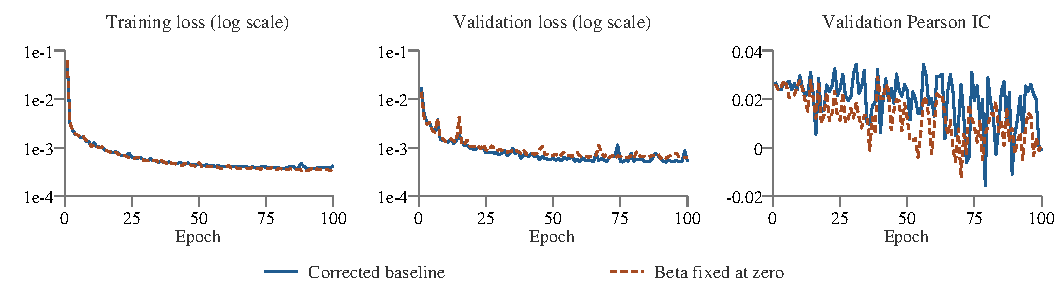
\includegraphics[width=0.94\textwidth]{learning_curves.pdf}
\caption{Corrected-sampler eager-FP32 seed-0 trajectories from saved logs. Loss panels share logarithmic axes.}
\label{fig:learning}
\end{figure*}
\begin{figure*}[t]
\centering
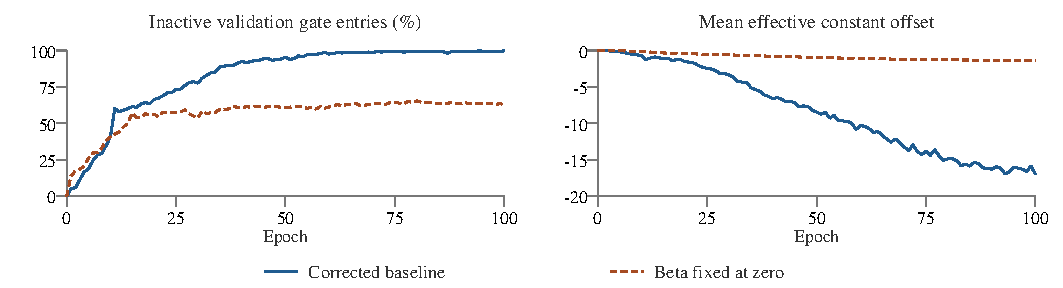
\includegraphics[width=0.94\textwidth]{mechanism_figure.pdf}
\caption{Matched seed-0 fixed-probe inactivity and effective-offset trajectories, distinct from full-period censuses.}
\label{fig:mechanism}
\end{figure*}

Table~\ref{tab:beta} separates the activation outcome from the forecasting outcome. At selected beta-zero states, all 20 units retain some validation activity and no validation window is wholly inactive. Test IC increases from 0.02848 to 0.03053 for seed 0, but decreases from 0.02742 to 0.01244 for seed 1. Preventing near-total shutdown therefore does not consistently improve forecasting. Other learned parameters and representation changes remain relevant even after the additive normalization bias is fixed.

In Figure~\ref{fig:learning}, loss falls sharply early while validation IC fluctuates later. Figure~\ref{fig:mechanism} shows persistent beta-zero separation in activity and effective offset, agreeing with the selected-state censuses. Forecasting gains still differ by seed.

\balance
\subsection{Discussion and Limitations}
The saved records allow each selected checkpoint to be recovered. Fixed probes show when branch activity changes, and full-period censuses establish how widely that behavior occurs. Matching initial values and shuffle sequences makes the beta intervention interpretable within this protocol. Generalization to other StockMixer settings requires further matched runs.

Main experiments preserve the released overlap, while corrective experiments remove target reuse. Sampling and precision changed together when establishing the clean FP32 baseline, so their individual causal effects are not isolated by that comparison. Beta-zero is subsequently tested within matched corrected settings. The current environment differs from the historical release stack and GPU determinism was not enforced~\cite{torchrepro}. Missing exact paper ablation sources are an implementation uncertainty, not an established cause of lower scores. The test period has already been inspected; follow-up results are exploratory and across-run variation is descriptive rather than proof of statistical significance.

\section{Conclusion and Future Work}
This project combines StockMixer reproduction with exact recording, recoverable weights, full-state resumption, execution analysis, and branch diagnostics. Across 21 main runs and 2,100 epochs, released HardSwish records IC 0.0408 and modified no-stock reaches mean IC 0.03517. Error, correlation, precision, and portfolio Sharpe capture different forecasting properties.

Learned beta contributes to a large negative stock-MLP offset. Freezing it restores substantial activation coverage without consistently improving prediction. The 9--9 tolerance-selection result leaves the value of that checkpoint rule unresolved. Saving the states still provides a practical benefit: the selections and internal behavior can be checked after training.

Future work should complete execution-matched repetitions with initial-weight and shuffle records, then evaluate a fresh period with transaction costs and portfolio-size sensitivity. NYSE/S\&P500 expansion and separate sampling, precision, and normalization interventions would test generality. Fresh-period evaluation and matched repetitions would address the current differences in execution settings and the retained training/validation overlap.

\begin{thebibliography}{9}
\bibitem{stockmixer} J. Fan and Y. Shen, ``StockMixer: A simple yet strong MLP-based architecture for stock price forecasting,'' in \emph{Proc. AAAI Conf. Artif. Intell.}, vol. 38, no. 8, pp. 8389--8397, 2024, doi: 10.1609/aaai.v38i8.28681.
\bibitem{mlpmixer} I. Tolstikhin \emph{et al.}, ``MLP-Mixer: An all-MLP architecture for vision,'' in \emph{Advances in Neural Information Processing Systems}, vol. 34, pp. 24261--24272, 2021.
\bibitem{lstm} S. Hochreiter and J. Schmidhuber, ``Long short-term memory,'' \emph{Neural Computation}, vol. 9, no. 8, pp. 1735--1780, 1997, doi: 10.1162/neco.1997.9.8.1735.
\bibitem{gru} K. Cho \emph{et al.}, ``Learning phrase representations using RNN encoder--decoder for statistical machine translation,'' in \emph{Proc. EMNLP}, pp. 1724--1734, 2014, doi: 10.3115/v1/D14-1179.
\bibitem{rsr} F. Feng, X. He, X. Wang, C. Luo, Y. Liu, and T.-S. Chua, ``Temporal relational ranking for stock prediction,'' \emph{ACM Trans. Inf. Syst.}, vol. 37, no. 2, Art. no. 27, pp. 1--30, 2019, doi: 10.1145/3309547.
\bibitem{releasedcode} SJTU-DMTai, ``StockMixer released source,'' revision cce13598afd3ff33ae317700a85ae08db0554652. [Online]. Available: \url{https://github.com/SJTU-DMTai/StockMixer}
\bibitem{project} K. K. Yuvaraj, ``StockMixer project experiment archive: NASDAQ logs, checkpoints, configurations, and diagnostics,'' unpublished project materials, 2026. Project repository: \url{https://github.com/artemiskavin/Stock-Mixer}.
\bibitem{torchrepro} PyTorch Contributors, ``Reproducibility,'' \emph{PyTorch 2.9 Documentation}. Accessed: Nov. 1, 2026. [Online]. Available: \url{https://docs.pytorch.org/docs/2.9/notes/randomness.html}
\end{thebibliography}

\end{document}
